\EnglishSourceFrame{GELFAND-P001455}{49}
\begin{center}
\begin{tikzpicture}[x=0.012cm,y=-0.012cm,line width=0.5pt]
\node at (145,215) {(10)};
\draw (255,217)--(256,160)--(310,87);
\draw (345,78)--(425,72)--(510,107)--(555,160)--(550,216)--(527,270);
\draw (507,303)--(402,321);
\draw (315,278)--(280,269)--(256,231);
\draw (360,155)--(410,200);
\draw (402,250)--(472,210);
\draw (550,216)..controls (620,196) and (652,394)..(539,429)..controls (480,426) and (433,376)..(402,321);
\draw (550,216) circle (6);
\draw (402,321) circle (6);
\node at (600,186) {$1$};
\node at (390,384) {$3$};
\end{tikzpicture}
\end{center}
Consider a more complicated configuration
and all possible colourings of the boundary
(with 4 colours).

Some extend to the interior,
and some do not.

One can try recolourings as in (9) (with pol. success [source abbreviation]).
In this way the computer searches for reducible configurations.

\begin{center}
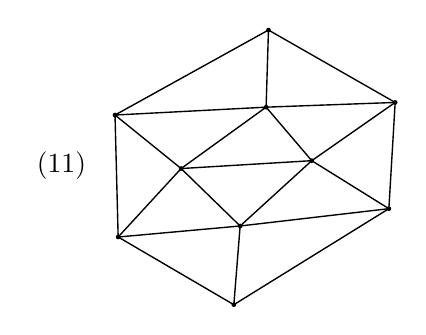
\begin{tikzpicture}[x=0.01cm,y=-0.01cm,line width=0.5pt]
\node at (335,870) {(11)};
\coordinate (a) at (598,698);
\coordinate (b) at (759,790);
\coordinate (c) at (751,925);
\coordinate (d) at (554,1047);
\coordinate (e) at (407,961);
\coordinate (f) at (403,806);
\coordinate (g) at (595,796);
\coordinate (h) at (487,874);
\coordinate (i) at (653,864);
\coordinate (j) at (562,947);
\draw (a)--(b)--(c)--(d)--(e)--(f)--(a);
\draw (a)--(g)--(b);
\draw (f)--(g)--(h)--(f);
\draw (h)--(e);
\draw (g)--(i)--(b);
\draw (h)--(i)--(c);
\draw (h)--(j)--(i);
\draw (e)--(j)--(c);
\draw (j)--(d);
\fill (a) circle (3);
\fill (b) circle (3);
\fill (c) circle (3);
\fill (d) circle (3);
\fill (e) circle (3);
\fill (f) circle (3);
\fill (g) circle (3);
\fill (h) circle (3);
\fill (i) circle (3);
\fill (j) circle (3);
\end{tikzpicture}
\end{center}
A reducible configuration
(but Fuchs [crossed out: \EnglishUnclear{GELFAND-P001455}{configuration-cancel}{u / d [source letters]}] did not manage to prove it).

I.M.G. \underline{Problem} \EnglishUnclear{GELFAND-P001455}{task-number}{6 / v [source letter]}.
Write a program to determine reducibility for
a parallel computer.

One of Appel and Haken's configurations (out of 1700) was checked
by hand (Allaire), because the machine could not handle it.

\underline{An unavoidable set.}

Their construction is based on Euler's theorem
\begin{equation*}
\mathrm{В}-\mathrm{Р}+\mathrm{Г}=2.\tag{12}
\end{equation*}
\underline{Kempe:} let \EnglishUnclear{GELFAND-P001455}{vertex-count-symbol}{$\nu_i$ / $v_i$} be the number of vertices connected to exactly
$i$ other vertices ($i$ edges leave them).
\begin{equation*}
\mathrm{В}=\nu_3+\nu_4+\nu_5+\ldots\tag{13}
\end{equation*}
\begin{equation*}
\mathrm{Р}=\frac{1}{2}(3\nu_3+4\nu_4+5\nu_5+\ldots)\tag{14}
\end{equation*}
\begin{center}
\begin{tikzpicture}[x=0.01cm,y=-0.01cm,line width=0.5pt]
\draw (298,2590) circle (5);
\draw (302,2585)--(430,2520);
\end{tikzpicture}
\end{center}
\begin{equation*}
2\mathrm{Р}=\text{number of such pairs}=3\nu_3+4\nu_4+\ldots
\end{equation*}
(a vertex and an edge leaving it)
\begin{equation*}
3\mathrm{Г}=2\mathrm{Р}\qquad\text{(since this is a triangulation)}\tag{15}
\end{equation*}
hence
\begin{equation*}
\mathrm{Г}=\frac{3\nu_3+4\nu_4+5\nu_5+\ldots}{3}\tag{15'}
\end{equation*}
From (12) we find:
\begin{equation*}
3\nu_3+2\nu_4+\nu_5-\nu_7-2\nu_8-3\nu_9-\ldots=12,\tag{16}
\end{equation*}
i.e.

[Crossed-out number: \EnglishUnclear{GELFAND-P001455}{cancelled-equation-number}{(17) / (16)}]
\begin{equation*}
\sum_{i=3}^{\infty}(6-i)\nu_i=12\tag{16'}
\end{equation*}

\par\smallskip\noindent\leavevmode\phantomsection\label{GELFAND-P001455:recolouring-success-abbreviation:editorial}{\footnotesize\textbf{Editorial comparison.} The source writes “с пол. успех.” The abbreviation “пол.” was checked at 3×, 5× and 10×. Its expansion to “full” or “partial” is not established; the translation retains “pol.” with an explicit source-abbreviation marker.\par}\smallskip


\EnglishSourceFrame{GELFAND-P001456}{unlabelled}
(17) Hence one of the numbers \EnglishUnclear{GELFAND-P001456}{vertex-count-symbol}{$\nu_3,\nu_4,\nu_5$ / $v_3,v_4,v_5$} is different from $0$.

We obtain an unavoidable set

\begin{center}
\begin{tikzpicture}[x=0.018cm,y=-0.018cm,line width=0.5pt]
\node at (300,390) {(18)};
\draw (377,433)--(432,328)--(484,421)--(377,433);
\draw (377,433)--(430,391)--(484,421);
\draw[line width=1pt] (432,328)--(430,391);
\fill (430,391) circle (3);
\draw (405,490)--(405,550);
\node at (435,590) {reducible};
\draw (609,372)--(667,325)--(761,355)--(657,434)--(609,372);
\draw (609,372)--(761,355);
\draw (667,325)--(657,434);
\draw (685,490)--(685,550);
\node at (685,590) {reducible};
\end{tikzpicture}
\end{center}
\EnglishSourceFigure{GELFAND-P001456}{diagram-18-right}{The third drawing in (18): a pentagonal outline with an upper vertex, two side vertices and two lower vertices; an interior node has five segments to the vertices of the outline. The upper-right side is retraced with a dense wedge-shaped stroke; at its right end is a short projection whose nature is unclear. Below the drawing is a vertical pointer to the caption “cannot immediately / prove reducibility”.}

\par\medskip\noindent
\begin{minipage}[c]{0.48\linewidth}\centering
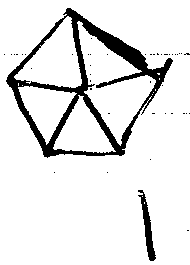
\includegraphics[width=\linewidth]{figures/gelfand-p001456-diagram-18-right-original-r2.png}
\par\smallskip{\footnotesize Original manuscript diagram: GELFAND-P001456\par}
\end{minipage}\hfill
\begin{minipage}[c]{0.48\linewidth}\centering
\resizebox{\linewidth}{!}{% Visible strokes only: the thick wedge is not asserted to be an arrow.
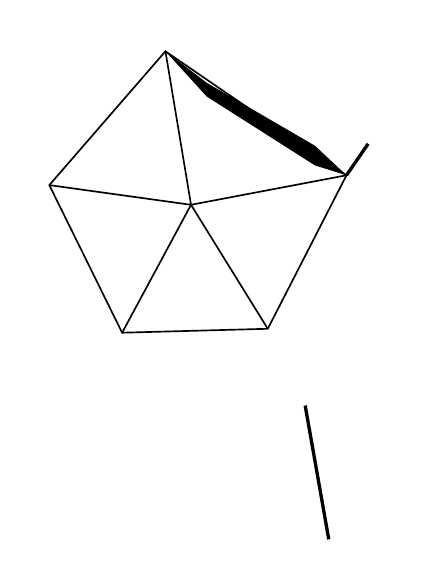
\begin{tikzpicture}[x=0.025cm,y=-0.025cm,line width=0.6pt]
\path[use as bounding box] (0,0) rectangle (190,265);
\draw (11,80)--(70,12)--(162,75)--(122,153)--(48,155)--cycle;
\draw (70,12)--(83,90)--(11,80);
\draw (48,155)--(83,90)--(122,153);
\draw (83,90)--(162,75);
\fill (70,12)--(91,28)--(146,60)--(162,75)--(146,70)--(91,35)--cycle;
\draw[line width=1.2pt] (162,75)--(173,59);
\draw[line width=1.2pt] (141,192)--(153,260);
\end{tikzpicture}
}
\par\smallskip{\footnotesize Partial recreation of visible strokes; uncertain joins and labels remain explicit.\par}
\end{minipage}\par\medskip


Now one may consider only triangulations with
\begin{equation*}
\nu_3=\nu_4=0\tag{19}
\end{equation*}
\underline{Discharging}

(20) Initial charge: to a vertex from which $i$ edges leave,
assign the charge [crossed out: \EnglishUnclear{GELFAND-P001456}{initial-charge-cancel}{$60-i$ / $6-i$}] $60(6-i)$.

\underline{Recharging procedure:} construct another function on the vertices.
\begin{equation*}
(16')\Longleftrightarrow\text{sum of all charges}=720.
\end{equation*}
(21) We want [inserted above: “to make”] all charges $\leq0$.

(which is impossible [crossed out: \EnglishUnclear{GELFAND-P001456}{impossible-cancel}{illegible}] in view of equality (16'))

\underline{Procedure 1.}

\begin{center}
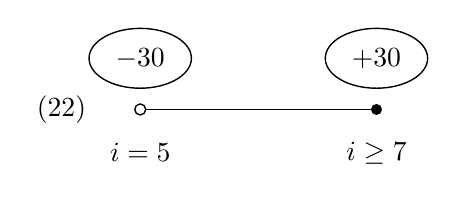
\begin{tikzpicture}[line width=0.5pt]
\node at (-1,0) {(22)};
\draw (0.07,0)--(3,0);
\draw (0,0) circle (0.07);
\fill (3,0) circle (0.07);
\draw (0,0.65) ellipse (0.65 and 0.38);
\node at (0,0.65) {$-30$};
\draw (3,0.65) ellipse (0.65 and 0.38);
\node at (3,0.65) {$+30$};
\node at (0,-0.55) {$i=5$};
\node at (3,-0.55) {$i\geq7$};
\end{tikzpicture}
\end{center}
(at the 1st vertex we decrease by 30,
at the 2nd we increase by 30)

\underline{Several situations in which a positive charge remains somewhere}

(23) $1^{\circ}$.
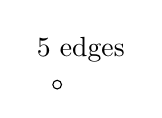
\begin{tikzpicture}[baseline=0pt]
\draw (0,0) circle (0.055);
\node at (0.3,0.45) {5 edges};
\end{tikzpicture}
is connected to $0$ or $1$ [crossed out: \EnglishUnclear{GELFAND-P001456}{situation-one-cancel}{edges [source abbreviated form] / edges [source full form]}] vertices with number of edges $\geq7$.

($\Rightarrow$ a vertex with positive charge remains

[A separately crossed-out sign: \EnglishUnclear{GELFAND-P001456}{cancelled-enumeration}{2 / illegible}]

(24) $2^{\circ}$.
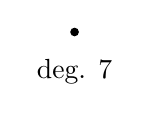
\begin{tikzpicture}[baseline=0pt]
\fill (0,0) circle (0.055);
\node at (0,-0.5) {deg. 7};
\end{tikzpicture}
is connected [crossed out: \EnglishUnclear{GELFAND-P001456}{situation-two-cancel}{edges with / an edge with}] to $\leq2$ vertices of degree $5$.

Eventually a finite set of configurations is obtained that is unavoidable,
because if none of them occurs, all
charges can be made $\leq0$.

\par\smallskip\noindent\leavevmode\phantomsection\label{GELFAND-P001456:case24-charge-inequality:editorial}{\footnotesize\textbf{Editorial comparison.} The source relation in case (24) is $\le2$, confirmed at 3×, 5× and 10×. Under the written transfer of 30 per incident vertex of valency 5, the charge at a vertex of valency 7 is $-60+30k$, which is nonpositive when $k\le2$. This local calculation does not give positive charge at that vertex. It neither disproves the wider claim of positive charge somewhere nor licenses a replacement by $\ge3$.\par}\smallskip


\EnglishSourceFrame{GELFAND-P001457}{50}
Now their reducibility must be checked.

The authors (Appel and Haken) in 1977 thank the administration
for 12000 hours of machine time.
[The number 12000 has a wavy underline; below it: “(1200?)”.]

The configurations are then transformed into more complicated ones,
and so are the transfer rules.

\underline{\underline{A. Beilinson}} (continuation)

(on work by K. Vilonen, S. Gelfand, R. D. MacPherson)

[Below “D.”, with a pointer: “Duncan”.]

$X$ is a smooth [inserted above: “complex”] algebraic variety,

$\mathcal{F}$ is a finite-dimensional constructible [crossed out: “sheaf”; replacement above: “complex of sheaves”] on $X$.

From these data one constructs

$\mathrm{SS}(\mathcal{F})$, a Lagrangian conic variety in
[crossed out: $T^*X$] $\Omega X=T^*X$.

$\mathrm{SS}(\mathcal{F})=\text{zero section}\Longleftrightarrow H^i(\mathcal{F})$ is smooth, i.e. locally constant.

\underline{Definition.} $\mathrm{SS}\mathcal{F}$

\begin{equation*}
H^\bullet(\mathcal{F})=0\quad\Rightarrow\quad\mathrm{SS}(\mathcal{F})=\varnothing\tag{1}
\end{equation*}
\begin{equation*}
H^\bullet(\mathcal{F})\neq0\quad\Rightarrow\quad\mathrm{SS}(\mathcal{F})\supset\text{zero section},\quad\text{and}
\end{equation*}
$\mathrm{SS}(\mathcal{F})\setminus(\text{zero section})$ is described as follows.
\begin{equation*}
\nu\in\Omega_x^1,\qquad\text{choose }f:\quad df_x=\nu,\quad f(x)=0
\end{equation*}
[Below $\nu$, with a pointer: “vector”.]

Let $U$ be a small neighbourhood of the point $x$.
\begin{equation*}
H^\bullet(U,U\cap f^{-1}(\varepsilon)\text{[crossed out: }\mathcal{F}\text{]};\mathcal{F})
=\Phi_f^\bullet(\mathcal{F})_x\tag{2}
\end{equation*}
(the space of vanishing [crossed out: \EnglishUnclear{GELFAND-P001457}{vanishing-cycles-cancel}{cocycles / cohomol.}] cycles)

$\varepsilon\neq0$ is small.

(\EnglishUnclear{GELFAND-P001457}{hypercohomology-word}{hyperhomology / hypercohomology})

(relative cohomology is defined through the cone)
of the map, i.e. one must write a bicomplex and
totalize it.

\begin{equation*}
\begin{tikzcd}
\mathcal{F}^1(U) \arrow[r] & \mathcal{F}^1(U\cap f^{-1}(\varepsilon)) \\
\mathcal{F}^0(U) \arrow[r] \arrow[u] & \mathcal{F}^0(U\cap f^{-1}(\varepsilon)) \arrow[u]
\end{tikzcd}
\end{equation*}
(if $\mathcal{F}$ is sufficiently
acyclic)

\EnglishSourceFrame{GELFAND-P001458}{unlabelled}
An explanation of [crossed out: \EnglishUnclear{GELFAND-P001458}{top-cancellation}{why / what for}; inserted above: how] vanishing cycles enter here.

\EnglishSourceFigure{GELFAND-P001458}{vanishing-cycle-sketch}{At the upper left, several arcs meet at one point; on the right, a narrow hatched oval lies between two arcs. Below is a horizontal oval with two points joined by a stroke with a head at the left point. A broken line runs from the upper-right oval to the lower-right point. The exact geometry and direction of individual strokes require comparison with the original.}

\par\medskip\noindent
\begin{minipage}[c]{0.48\linewidth}\centering
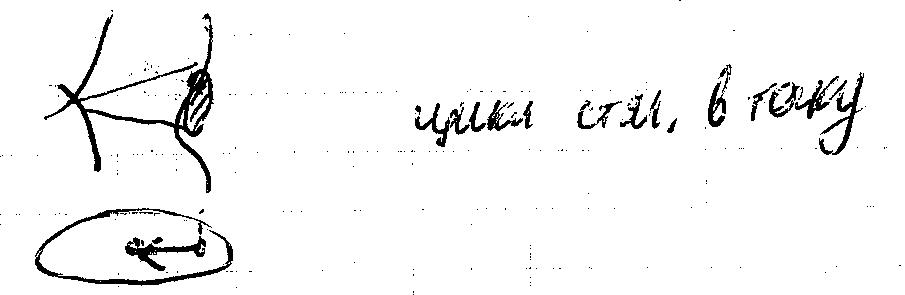
\includegraphics[width=\linewidth]{figures/gelfand-p001458-vanishing-cycle-sketch-original.png}
\par\smallskip{\footnotesize Original manuscript diagram: GELFAND-P001458\par}
\end{minipage}\hfill
\begin{minipage}[c]{0.48\linewidth}\centering
\resizebox{\linewidth}{!}{\def\VanishingCycleCaption{cycle contracts [source abbreviation unresolved] to a point}
% Partial trace: hatching, lower left head and broken vertical strokes retained.
\begin{tikzpicture}[x=0.01cm,y=-0.01cm,line width=0.55pt]
\path[use as bounding box] (0,0) rectangle (905,295);
\draw (45,86)--(75,102)--(45,118);
\draw (75,102)..controls(92,76)and(103,35)..(112,13);
\draw (75,102)..controls(88,124)and(95,149)..(98,170);
\draw (75,102)--(200,65);
\draw (75,102)..controls(111,122)and(149,125)..(185,130);
\draw (207,15)..controls(218,35)and(205,65)..(200,65);
\draw (200,65)..controls(217,84)and(215,117)..(191,136)
 ..controls(170,135)and(176,109)..(188,84)..controls(195,76)and(198,70)..(200,65);
\draw (191,136)..controls(205,151)and(212,173)..(208,190);
\draw (189,89)--(204,74);\draw (182,107)--(208,79);
\draw (179,123)--(209,92);\draw (184,132)--(204,108);
\draw (132,249) ellipse [x radius=99,y radius=37];
\fill (140,250) circle[radius=2];\fill (199,249) circle[radius=2];
\draw (140,250)--(199,249);\draw (154,242)--(140,250)--(160,268);
\draw (200,210)--(200,217);\draw (199,225)--(199,233);\draw (199,240)--(199,245);
\node[anchor=west,text width=4.5cm,align=left] at (400,110) {\VanishingCycleCaption};
\end{tikzpicture}
}
\par\smallskip{\footnotesize Partial recreation of visible strokes; uncertain joins and labels remain explicit.\par}
\end{minipage}\par\medskip


[To the right of the drawing:] the cycle \EnglishUnclear{GELFAND-P001458}{cycle-caption}{contracts [two possible source abbreviations]} to a point.

\underline{Df.} $\nu\notin SS(\mathcal F)\Longleftrightarrow$ the vanishing cycles at $\nu$ are $0$, i.e. \EnglishUnclear{GELFAND-P001458}{vanishing-cycles-degree}{$\Phi_f^i(\mathcal F)_x=0$ / $\Phi_f^\bullet(\mathcal F)_x=0$ / $\Phi_f^*(\mathcal F)_x=0$}.

Consider the direct image of $\mathcal F|_U$ under the map $U\overset{f}{\longrightarrow}\text{disk}$.

Vanishing cycles measure how the fibre at $0$ differs from neighbouring fibres.

$f$ is called a \underline{Morse} function on $X$ if [inserted above: $f$ is a holomorphic function on $X$ and] the graph $df(X)\subset$ [crossed out: \EnglishUnclear{GELFAND-P001458}{cotangent-cancellation}{an illegible sign}] $\Omega^1$ intersects $SS(\mathcal F)$ transversely.

A complex is called a \underline{perverse sheaf} if for $\forall$ functions that are Morse with respect to $\mathcal F$ there are vanishing cycles only in dimension $0$.

(only $\Phi_f^0(\mathcal F)\neq0$)

$\mathcal F$ is a perverse sheaf.

From it one constructs a \underline{local system on the regular points of the singular support}.

Its fibre over the point $\nu$ is:
\begin{equation*}
\Phi(\mathcal F)_\nu=\Phi_f^0(\mathcal F)_x
\end{equation*}
for a Morse function $f$ with $df(x)=\nu$, \EnglishUnclear{GELFAND-P001458}{normalization-argument}{$f(0)=0$}.

What happens at singular points?

\underline{Problem}: describe perverse sheaves microlocally,
i.e. in terms of vanishing cycles.

The paper solves half of it.

\underline{Meaning}: where do perverse sheaves come from?

$1^\circ$. $\mathcal M$ is an overdetermined system.

[Below “system”:] (holon.)

[On the right:] $\sum f_i\partial^i$

[Below $f_i$, a vertical line to the caption:] holom.

\begin{equation*}
\mathcal F^{0,0}\overset{\bar\partial}{\longrightarrow}\mathcal F^{0,1}\longrightarrow\cdots
\end{equation*}

[A separate sign above the beginning of the next line:] \EnglishUnclear{GELFAND-P001458}{lower-detached-mark}{4 / insertion mark}

if $u\in\mathcal F^{0,0}$ is a solution of $\mathcal M$, then so is $\bar\partial u$.

The system is overdetermined, $\Rightarrow$ the complex of solutions is a perverse sheaf.

\EnglishSourceFrame{GELFAND-P001459}{51}
$2^\circ$. The combinatorial method

(Goresky--MacPherson)

There is [inserted above: a general] method for extending sheaves to singular points $\Rightarrow$ one obtains [crossed out: \EnglishUnclear{GELFAND-P001459}{upper-cancellation}{an illegible word}] perverse sheaves.

The paper is devoted to the $3$rd method.

\underline{Next time} $(18/\mathrm{IV})$: a talk by \underline{Reshetikhin} on quantum groups.

[Below is a horizontal line. Beneath it, at the lower edge of the text fragment: \EnglishUnclear{GELFAND-P001459}{bottom-cutoff}{cropped strokes, possibly “M…”}.]

\EnglishSourceFrame{GELFAND-P001460}{unlabelled}
\underline{18.4.1988}\qquad \underline{\underline{Gelfand's seminar.}}

[The following heading has a wavy underline; the author names in the left margin have broken underlines.]
\underline{Titles of Bourbaki seminar talks} $(87-88\text{ year})$

\underline{Lerner.}\quad "The uncertainty principle and microlocalization" (after Fefferman and Phong)

"Geometry of polynomials and Newton's method" (after Smale and Shub)

"Mixed nonlinear problems"

"Noncommutative stochastic calculus"

"The metaplectic representation and Howe's conjecture"

"The Schottky problem and Novikov's conjecture"

\underline{Douady.}\quad "Siegel disks and the Herman ring"

"Deformations of plane curves"

"Large deviations"

"Classification of unitary representations of real groups"

"Classification theory"

"Stable sheaves and [crossed out: \EnglishUnclear{GELFAND-P001460}{stable-cancellation}{an illegible word}]
[No clear closing quotation mark survives after the cancelled material.]

"Moonshine"

\underline{Verdier.}\quad "Quantum groups\EnglishUnclear{GELFAND-P001460}{quantum-title-mark}{[superscript sign: crossed-out quotation marks / an asterisk]} (after Drinfeld)"

\underline{Malgrange.}\quad "The geometric Fourier transform"

"New invariants of homology spheres of dimension $3$"

"Elliptic cohomology"

"Recent advances on Fermat's theorem".

\EnglishSourceFrame{GELFAND-P001461}{63}
[The surname has a straight underline; “on work by Atiyah” has a wavy underline.]
\underline{Beilinson} \underline{on work by Atiyah} and someone else.

\underline{Semi-infinite Morse theory.}

In the $\infty$-dimensional case there are 2 versions of Morse theory (for computing homology).

1) The geodesic problem with the energy functional resembles the finite-dimensional case.
The negative index of inertia is finite and equals the number of conjugate points on the geodesic.

2) An $\infty$-dimensional manifold, an energy-type functional
with isolated critical points, but with an $\infty$ number of $+$ and an $\infty$ number of $-$.
But it turns out that for two different critical points the number of $-$ differs by a finite
number; homology is constructed, counted from $\infty/2$
(a topological version of Feigin and Tsygan).

[“Sensation” has a wavy underline.]
\underline{Sensation}: these invariants are related to Donaldson invariants
of 4-dimensional manifolds.

\begin{center}
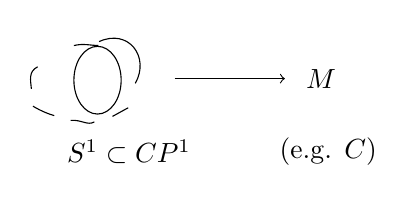
\begin{tikzpicture}[x=1cm,y=1cm]
\draw (0,0) ellipse (0.30 and 0.43);
\draw (-0.30,0.44) .. controls (-0.18,0.47) and (-0.08,0.44) .. (0.01,0.44);
\draw (0.02,0.49) .. controls (0.39,0.66) and (0.67,0.30) .. (0.48,-0.04);
\draw (-0.76,0.17) .. controls (-0.88,0.11) and (-0.85,0.00) .. (-0.84,-0.11);
\draw (-0.82,-0.33) .. controls (-0.72,-0.39) and (-0.62,-0.43) .. (-0.55,-0.45);
\draw (-0.34,-0.51) .. controls (-0.20,-0.50) and (-0.13,-0.58) .. (-0.04,-0.53);
\draw (0.19,-0.46) -- (0.39,-0.35);
\draw[->] (0.98,0.02) -- (2.38,0.02);
\node at (2.84,0.02) {$M$};
\node at (0.40,-0.91) {$S^1\subset\mathbb C P^1$};
\node at (2.93,-0.91) {(e.g. $\mathbb C$)};
\end{tikzpicture}
\end{center}

For $S^1\to\mathbb C$, select 2 halves (extension to the inside and outside);
they intersect in a finite-dimensional manifold.

\EnglishSourceFigure{GELFAND-P001461}{surface-sketch}{On the left is an oval outline with two small loop-like strokes inside; outside is a wider, partly dashed outline. The exact join of the upper internal stroke to the outline and the meaning of the internal loops require comparison with the original.}

\par\medskip\noindent
\begin{minipage}[c]{0.48\linewidth}\centering
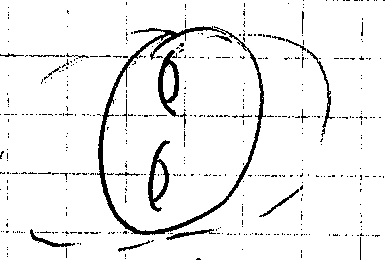
\includegraphics[width=\linewidth]{figures/gelfand-p001461-surface-sketch-original-r2.png}
\par\smallskip{\footnotesize Original manuscript diagram: GELFAND-P001461\par}
\end{minipage}\hfill
\begin{minipage}[c]{0.48\linewidth}\centering
\resizebox{\linewidth}{!}{% Partial stroke trace; no genus, handle attachment or missing join is inferred.
\begin{tikzpicture}[x=0.02cm,y=-0.02cm,line width=0.55pt]
\path[use as bounding box] (0,0) rectangle (385,260);
\draw (190,30)..controls(145,34)and(112,95)..(100,155)
 ..controls(92,196)and(100,220)..(130,230)
 ..controls(165,242)and(220,205)..(241,158)
 ..controls(269,103)and(268,59)..(235,40)..controls(221,27)and(204,28)..(190,30);
\draw (174,53)..controls(156,67)and(153,85)..(160,103)
 ..controls(168,118)and(179,103)..(177,78)..controls(174,67)and(169,61)..(168,61);
\draw (160,103)..controls(164,110)and(169,113)..(176,116);
\draw (169,141)..controls(155,143)and(149,169)..(150,193)
 ..controls(151,207)and(159,214)..(163,207);
\draw (159,159)..controls(177,174)and(171,187)..(151,201);
\draw (131,34)..controls(144,28)and(164,28)..(178,32);
\draw (240,35)..controls(288,35)and(329,47)..(329,92);
\draw (329,94)..controls(334,112)and(326,130)..(323,143);
\draw (300,186)--(273,207)--(260,214);
\draw (250,231)--(200,240);\draw (155,237)--(120,247);
\draw (94,242)--(68,244)--(32,235);\draw (42,81)--(63,66);
\end{tikzpicture}
}
\par\smallskip{\footnotesize Partial recreation of visible strokes; uncertain joins and labels remain explicit.\par}
\end{minipage}\par\medskip

[Below the drawing:] Riemann surface $\subset$ sphere.

[To the right of the drawing:] gauge fields; the Yang--Mills functional.
Critical points are flat connections.

\underline{I.M.G.} We made use of the decomposition of $C^\infty(S^1)$ ($\sim20$ years)
(including Hirota--Sato $\tau$-functions, $\frac12$-cohomology).

It is remarkable that $S^1$ can be replaced by other manifolds.
This will be discussed next time.

\underline{\underline{Reshetikhin}} \underline{Kolya}.

[Crossed out and underlined: Quantum groups.]

$\underline{U_q(SU(2))}$ \underline{and link invariants and representations of the braid group.}

\begin{equation*}
A=\underset{\text{associative algebra}}{U_q(SU(2))};\qquad
1,H,X^\pm\quad\text{--- generators}
\end{equation*}
\begin{equation*}
[X^\pm,H]=\mp2X^\pm;
\tag{1}
\end{equation*}
\begin{equation*}
[X^+,X^-]=\frac{\operatorname{sh}\left(\frac h2 H\right)}{\operatorname{sh}(h/2)};
\qquad q=e^h
\end{equation*}

\EnglishSourceFrame{GELFAND-P001462}{unlabelled}
[The basis monomial has a wavy underline in the source.]
\begin{equation*}
\underline{\left(q^{H/4}\right)^\ell H^n(X^+)^m(X^-)^k}
\quad\text{--- a vector-space basis}
\tag{2}
\end{equation*}

\begin{equation*}
\Delta:A\to A\otimes A
\end{equation*}
\begin{equation*}
\Delta(H)=H\otimes1+1\otimes H
\tag{3}
\end{equation*}
\begin{equation*}
\Delta(X^\pm)=X^\pm\otimes q^{H/4}+q^{-H/4}\otimes X^\pm
\end{equation*}

1. $\Delta$ is an algebra homomorphism. $\Delta(ab)=\Delta(a)\Delta(b)$

2. $\Delta$ is coassociative, i.e.
\begin{center}
\begin{tikzcd}[column sep=large,row sep=large]
& A\otimes A \arrow[dr,"\mathrm{id}\otimes\Delta"] & \\
A \arrow[ur,"\Delta"] \arrow[dr,"\Delta"'] & & A\otimes A\otimes A \\
& A\otimes A \arrow[ur,"\Delta\otimes\mathrm{id}"'] &
\end{tikzcd}
\end{center}
[On the right:] (Hopf algebra)

3. [Crossed out: \EnglishUnclear{GELFAND-P001462}{antipode-cancelled-sign}{an illegible sign}.]
$S:A\to A$ is an antihomomorphism (analogous to passing to the inverse
element in the algebra of functions on a group).

\begin{equation*}
S(X^\pm)=q^{H/2}X^\pm q^{-H/2}
\tag{4}
\end{equation*}
\EnglishUnclear{GELFAND-P001462}{antipode-formula}{[Formula (4): as in the source.]}
\begin{equation*}
S(H)=-H
\end{equation*}
\begin{equation*}
\epsilon(H)=\epsilon(X^\pm)=0
\end{equation*}

\begin{center}
\begin{tikzcd}[column sep=large,row sep=large]
& A\otimes A \arrow[r,shift left=1.2ex,"S\otimes\mathrm{id}"] \arrow[r,shift right=1.2ex,"\mathrm{id}\otimes S"'] & A\otimes A \arrow[dr,"m"] & \\
A \arrow[ur,"\Delta"] \arrow[drr,"\epsilon"'] & & & A \\
& & \mathbb C \arrow[ur,"e"'] &
\end{tikzcd}
\end{center}
[On the right:] (either arrow can be taken)

Transform it into a quadratic algebra in [inserted above: other] generators.
[Crossed out: \EnglishUnclear{GELFAND-P001462}{cancelled-generators}{possibly $K,X^\pm$, then illegible strokes}.]

Consider
\begin{equation*}
K=q^{H/2},\qquad K,X^\pm
\end{equation*}
[Crossed out on the left: $K,X^\pm$.]
\begin{equation*}
KX^\pm=q^{\pm1}X^\pm K
\end{equation*}
\begin{equation*}
X^+X^- -X^-X^+=\frac{K-K^{-1}}{q-q^{-1}}
\end{equation*}
\EnglishUnclear{GELFAND-P001462}{commutator-normalization}{[Denominator $q-q^{-1}$: as in the source.]}

\EnglishSourceFrame{GELFAND-P001463}{64}

(5) Involution
\begin{equation*}
(X^+)^*=X^-,\qquad H^*=H
\end{equation*}

Finite-dimensional representations
\begin{equation*}
\pi_j(X^{\pm})e_m^j=
\sqrt{\frac{\operatorname{sh}\bigl(\frac h2(j\mp m)\bigr)
\operatorname{sh}\bigl(\frac h2(j\pm m+1)\bigr)}
{\operatorname{sh}^{2}\bigl(\frac h2\bigr)}}\,e_{m\pm1},
\qquad j\in\mathbb Z/2,
\qquad -j\le m\le j
\tag{6}
\end{equation*}
\begin{equation*}
\dim V^j=2j+1\quad\text{(as for $\mathrm{SL}_2$)}
\end{equation*}

Sklyanin wrote in terms of quadratic algebras.

\underline{Exercise.} \underline{(I.M.G.)} $q=1\ \Rightarrow$ the formulas from the book by Gelfand--Minlos--Shapiro.

[On the right, set off by a bracket:] \underline{a concrete problem}: how to expand vector fields on the sphere in spherical \EnglishUnclear{GELFAND-P001463}{exercise-harmonics}{harmonics [two abbreviated source endings]}.

Begin with $\mathrm{SU}(2)$.

(7) \underline{Theorem.} Put
\begin{equation*}
R=\exp\left(\frac h4 H\otimes H\right)
\sum_{n\ge0}\frac{q^n}{[n]_q!}\,e^n\otimes f^n
\tag{8}
\end{equation*}
\EnglishUnclear{GELFAND-P001463}{r-coefficient}{Coefficient in (8): $q^n/[n]_q!$ [as written].}
\begin{equation*}
R\in U_q(\mathrm{SU}(2))^{\otimes2},
\end{equation*}
where
\begin{equation*}
e=q^{H/4}X^+,\qquad f=q^{-H/4}X^-,
\tag{9}
\end{equation*}

(10) 1.
\begin{equation*}
(\Delta\otimes\mathrm{id})R=R_{23}R_{13},
\qquad (\in U_q(\mathrm{SU}(2))^{\otimes3})
\end{equation*}
[Before the parenthesis on the right, crossed out: \EnglishUnclear{GELFAND-P001463}{cancelled-before-membership}{illegible}.]
\begin{equation*}
(\mathrm{id}\otimes\Delta)R=R_{12}R_{13};
\end{equation*}
\begin{equation*}
2.\quad \sigma\circ\Delta(a)=R\,\Delta(a)R^{-1};\qquad\text{(see (12))}
\end{equation*}
\begin{equation*}
3.\quad R_{12}R_{13}R_{23}=R_{23}R_{13}R_{12}.
\end{equation*}
[On the right:] (the Yang--Baxter equation with values in the tensor product of 3 copies of $A$)

In formula (8)
\begin{equation*}
[n]_q!=[n]_q\ldots[1]_q\qquad\text{($q$-factorial)}
\tag{11}
\end{equation*}

\underline{I.M.G.} Quantum mechanics is the right way to introduce $q$.

\underline{\underline{Exercise.}} What is $\Gamma_q$?

\begin{equation*}
\sigma\colon A^{\otimes2}\longrightarrow A^{\otimes2},\qquad
\sigma(f\otimes g)=g\otimes f
\tag{12}
\end{equation*}
In particular, $(10)_2$ implies that $\sigma\circ\Delta$ is also a comultiplication.

\EnglishSourceFrame{GELFAND-P001464}{unlabelled}

Define
\begin{equation*}
R^{j_1j_2}\colon V^{j_1}\otimes V^{j_2}\longrightarrow V^{j_2}\otimes V^{j_1}
\end{equation*}
\EnglishUnclear{GELFAND-P001464}{definition-separator}{After $R^{j_1j_2}$ is a corrected sign, $:$; the original strokes are illegible.}

$V^j$ is the space of a finite-dimensional representation.

\begin{equation*}
R^{j_1j_2}=P^{j_1j_2}\,\pi^{j_1}\otimes\pi^{j_2}(R)
\tag{13}
\end{equation*}
[Below $P^{j_1j_2}$, linked by a line:] the operator permuting the spaces.

\begin{equation*}
\begin{aligned}
&(1\otimes R^{j_1j_2})(R^{j_1j_3}\otimes1)(1\otimes R^{j_2j_3})=\\
&\qquad=(R^{j_2j_3}\otimes1)(1\otimes R^{j_1j_3})(R^{j_1j_2}\otimes1)
\end{aligned}
\tag{14}
\end{equation*}

$q$-analogues of [crossed out: \EnglishUnclear{GELFAND-P001464}{cancelled-coefficient}{an illegible sign}] Clebsch--Gordan coefficients.

All finite-dimensional representations are completely reducible.

\begin{equation*}
V^{j_1}\otimes V^{j_2}=\sum_{|j_1-j_2|\le j_3\le j_1+j_2}^{\oplus}V^{j_3}
\tag{15}
\end{equation*}
\EnglishUnclear{GELFAND-P001464}{sum-mark}{The sign above the sum is $\oplus$; possibly a correction from $\otimes$ to $\oplus$.}

$V_j$ was found by Kulish and Reshetikhin (1981).

In the basis:
\begin{equation*}
e_{m_1}^{j_1}\otimes e_{m_2}^{j_2}=
\sum_{|j_1-j_2|\le j_3\le j_1+j_2}
\begin{bmatrix}
j_1&j_2&j_3\\
m_1&m_2&m_3
\end{bmatrix}e_{m_3}^{j_3}
\tag{16}
\end{equation*}
[A line from the square bracket points to the caption:] Clebsch--Gordan coefficients.

where
\begin{equation*}
m_3=m_1+m_2
\end{equation*}

Graphical notation:
\begin{equation*}
A\colon V^{j_1}\otimes\ldots\otimes V^{j_N}
\longrightarrow V^{j'_1}\otimes\ldots\otimes V^{j'_L}
\end{equation*}

(17)
\begin{center}
\begin{tikzpicture}[x=1cm,y=1cm]
\draw (0,0.08)--(0,1.65)--(3.25,1.65)--(3.25,0)--(0,0);
\node at (1.63,0.82) {$A$};
\draw (0.35,1.65)--(0.35,2.55);
\draw (1.25,1.65)--(1.25,2.55);
\draw (3.1,1.65)--(3.1,2.55);
\node[left] at (0.25,2.28) {$j'_1$};
\node[left] at (1.15,2.28) {$j'_2$};
\node at (2.2,2.15) {$\ldots$};
\node[right] at (3.1,2.28) {$j'_L$};
\draw (0.4,0)--(0.4,-1);
\draw (1.35,0)--(1.35,-1);
\draw (2.97,0)--(2.97,-0.87);
\node[below] at (0.13,-1.04) {$j_1$};
\node[below] at (1.17,-1.04) {$j_2$};
\node[below] at (3.15,-1.04) {$j_N$};
\end{tikzpicture}
\end{center}

\begin{equation*}
A^{m'_1\ldots m'_N}_{m_1\ldots m_L}
\end{equation*}
\EnglishUnclear{GELFAND-P001464}{coefficient-range}{Coefficient indices: above, $m'_1\ldots m'_N$; below, $m_1\ldots m_L$ [as written].}
\begin{equation*}
-j_i\le m_i\le j_i;
\end{equation*}

[At the lower right:]
\EnglishSourceFigure{GELFAND-P001464}{diagram-02}{A rectangle containing $A$ with three vertical terminals above and below, without arrows. At the upper terminals: $j'_1$, $j'_2$, $j'_L$; above them: $m'_1$, $m'_2$, an ellipsis, and $m'$ with a corrected final index ($L$ or $N$). At the lower terminals: $j_1$, $j_2$, $j_N$; below them: $m_1$, $m_2$, $m_N$. The original sign beneath the corrected upper-right index requires checking.}

\par\medskip\noindent
\begin{minipage}[c]{0.48\linewidth}\centering
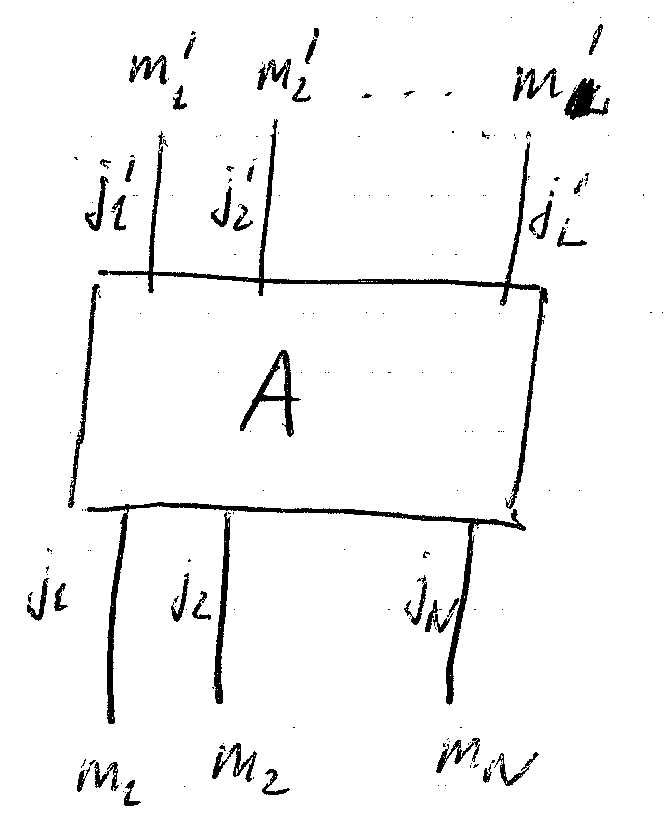
\includegraphics[width=\linewidth]{figures/gelfand-p001464-diagram-02-original.png}
\par\smallskip{\footnotesize Original manuscript diagram: GELFAND-P001464\par}
\end{minipage}\hfill
\begin{minipage}[c]{0.48\linewidth}\centering
\resizebox{\linewidth}{!}{% All clear source labels are typed. The overwritten last upper index stays uncertain.
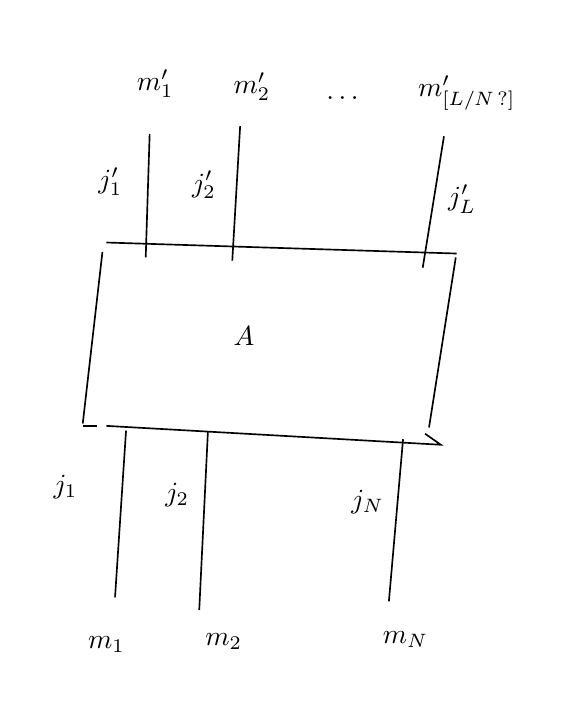
\begin{tikzpicture}[x=0.01cm,y=-0.01cm,line width=0.6pt]
\path[use as bounding box] (0,0) rectangle (665,830);
\draw (100,273)--(545,287);\draw (544,292)--(510,508);
\draw (505,516)--(525,530)--(100,506);\draw (88,506)--(70,506);
\draw (70,503)--(95,285);
\draw (155,135)--(150,292);\draw (270,125)--(260,296);\draw (529,138)--(502,305);
\draw (125,512)--(111,724);\draw (229,514)--(218,740);\draw (477,523)--(459,729);
\node at (275,392) {$A$};
\node at (105,196) {$j'_1$};\node at (224,200) {$j'_2$};\node at (552,218) {$j'_L$};
\node at (162,71) {$m'_1$};\node at (285,75) {$m'_2$};\node at (400,90) {$\ldots$};
\node at (558,83) {$m'_{[L/N\,?]}$};
\node at (48,584) {$j_1$};\node at (190,594) {$j_2$};\node at (432,603) {$j_N$};
\node at (100,784) {$m_1$};\node at (249,780) {$m_2$};\node at (480,778) {$m_N$};
\end{tikzpicture}
}
\par\smallskip{\footnotesize Partial recreation of visible strokes; uncertain joins and labels remain explicit.\par}
\end{minipage}\par\medskip


